\documentclass[a4paper, 10pt]{article}

\usepackage[default]{comfortaa}
\usepackage[utf8]{inputenc}
\usepackage[english]{babel}
\usepackage{graphicx}
\usepackage{geometry}
\usepackage{titlesec}
\usepackage{multicol}
\usepackage{lastpage}
\usepackage{fancyhdr}
\usepackage{array}
\usepackage{multirow, hhline}
\usepackage[table]{xcolor}
\usepackage[hidelinks]{hyperref}
\usepackage{textcomp}

\setlength{\columnseprule}{1pt}
\setlength{\columnsep}{1cm}

\definecolor{lightgray}{gray}{0.85}

\setlength{\arrayrulewidth}{0.35mm}
\setlength{\tabcolsep}{10pt}
\renewcommand{\arraystretch}{1.7}

\fancypagestyle{plain}{%
\fancyhf{} % clear all header and footer fields
\cfoot{\thepage /\pageref{LastPage}}
\rfoot{\href{https://github.com/ElectricCanary/FV1Buddy}{
\includegraphics[width=5mm, height=5mm]{github}}\hspace{8pt}\href{https://www.facebook.com/ElectricCanary}{
\includegraphics[width=5mm, height=5mm]{f}}\hspace{8pt}\href{https://www.instagram.com/electricanary/}{
\includegraphics[width=5mm, height=5mm]{inst}}\hspace{12pt}\href{mailto:support@electric-canary.com}{
\includegraphics[width=5mm, height=5mm]{email}}}
\lfoot{\textcolor{black!70}{{\footnotesize\textcopyright Electric Canary - June 2022}}}
\renewcommand{\headrulewidth}{0pt}
\renewcommand{\footrulewidth}{0pt}}


\pagestyle{fancy}
\renewcommand{\headrulewidth}{0pt}
\cfoot{}
\cfoot{\thepage /\pageref{LastPage}}
\rfoot{\href{https://github.com/ElectricCanary/FV1Buddy}{
\includegraphics[width=5mm, height=5mm]{github}}\hspace{8pt}\href{https://www.facebook.com/ElectricCanary}{
\includegraphics[width=5mm, height=5mm]{f}}\hspace{8pt}\href{https://www.instagram.com/electricanary/}{
\includegraphics[width=5mm, height=5mm]{inst}}\hspace{12pt}\href{mailto:support@electric-canary.com}{
\includegraphics[width=5mm, height=5mm]{email}}}
\lfoot{\textcolor{black!70}{{\footnotesize\textcopyright Electric Canary - June 2022}}}
\rhead{\href{https://electric-canary.com/FV1Buddy}{
\includegraphics[scale=0.22]{logo}}}
\lhead{\textbf{{\small\emph{\textcolor{black!70}{FV1Buddy-Datasheet}}}}}

\titleformat*{\section}{\huge\bfseries}
\titleformat*{\subsection}{\LARGE\bfseries}
\titleformat*{\subsubsection}{\Large\bfseries}

\geometry{hmargin=2.5cm,vmargin=2.5cm}
\headheight=35pt

\begin{document}\thispagestyle{plain}
\begin{center}
\begin{Huge}
\vspace*{0.5cm}
\textbf{FV1Buddy - Datasheet}
\rule {0.95\textwidth}{2pt}\\
\end{Huge}
\vspace{1cm}

\includegraphics[scale=1]{logocentre}\\
\end{center}
\vspace{1cm}
\begin{multicols}{2}
\section{Introduction}
\bigbreak

FV1Buddy is a Tap Tempo and Clock module for the Spin Semiconductor FV1 DSP.\\

This module is a great option for enabling tap tempo functionality in a FV1 based project.
The tap tempo is intuitive and has 6 different tempo divisions.\\
The clock output can also enhance the DSP's sound, unlike most circuits.\\
Other surprises like the momentary modulation and tempo save let's you enjoy your effects to the fullest.
\vfill\null
\columnbreak

\section{Features}
\bigbreak
\begin{itemize}
\item {Intuitive and Precise Tap Tempo}
\item \hyperref[subsec:tempodiv]{6 Selectable Tempo Divisions} \\ 
\includegraphics[scale=1]{fourth} , 
\includegraphics[scale=1]{dotted-eight} , 
\includegraphics[scale=1]{eight} , 
\includegraphics[scale=1]{triplet} , 
\includegraphics[scale=1]{sixteenth} , 
\includegraphics[scale=1]{sextuplet}
\item \hyperref[sec:clock]{48kHz Clock for Better Audio}
\item \hyperref[sec:temposave]{Tempo EEPROM Save}
\item \hyperref[subsec:ramp]{Ramp Modulation Momentary Effect}
\item \hyperref[sec:pinconfig]{Compact DIP-8 Package}
\item \hyperref[sec:typappsche]{No External Parts}
\item \hyperref[sec:calib]{Adjustable Maximum Delay}
\end{itemize}
\end{multicols}

\newpage
\headheight=35pt
\tableofcontents
\newpage

\section{Pin Configuration}
\label{sec:pinconfig}
\vfill
\begin{center}
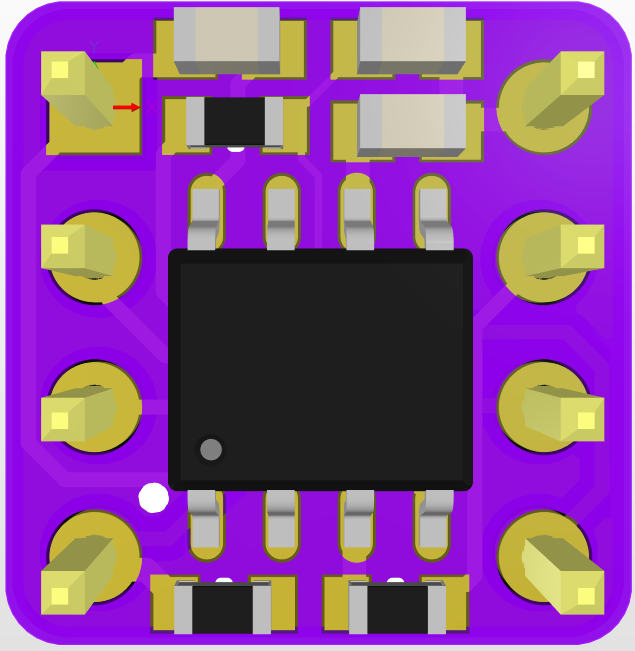
\includegraphics[scale=0.6]{FV1Buddy}
\vfill
\begin{table}[h!]
\begin{tabular}{|m{0.5cm}|m{4.5cm}|m{0.7cm}|m{7.5cm}|}
\hline
\rowcolor{lightgray} \centering {\Large\textbf{N°}} & \centering {\Large\textbf{Name}} & \centering {\Large\textbf{I/O}} & {\Large\textbf{Description}}\\
\hline
\centering 1 & \centering VCC & \centering I & Supply voltage.\\
\hline
\centering 2 & \centering Tap Button & \centering I & Set tempo when connected to ground.\\
\hline
\centering 3 & \centering Delay Time & \centering I & This pin's voltage determines the delay time when there's no tap sequence active.\\
\hline
\centering 4 & \centering Tempo Division Select & \centering I & This pin's voltage determines the tempo division selected.\\
\hline
\centering 5 & \centering Vout & \centering O & This pin can be connected to one of the pot pins of the FV1.\\
\hline
\centering 6 & \centering Clock Out & \centering O & 48kHz clock output for the FV1.\\
\hline
\centering 7 & \centering LED+ & \centering O & LED Indicator Output.\\
\hline
\centering 8 & \centering GND & \centering I & Ground.\\
\hline
\end{tabular}
\caption{Pin Configuration}
\end{table}
\end{center}
\vfill
\newpage

\section{Typical Application Schematic}
\label{sec:typappsche}
\bigbreak
This schematic shows how to implement the FV1Buddy into a simple delay project.
\vfill
\begin{figure} [h!]
\begin{center}
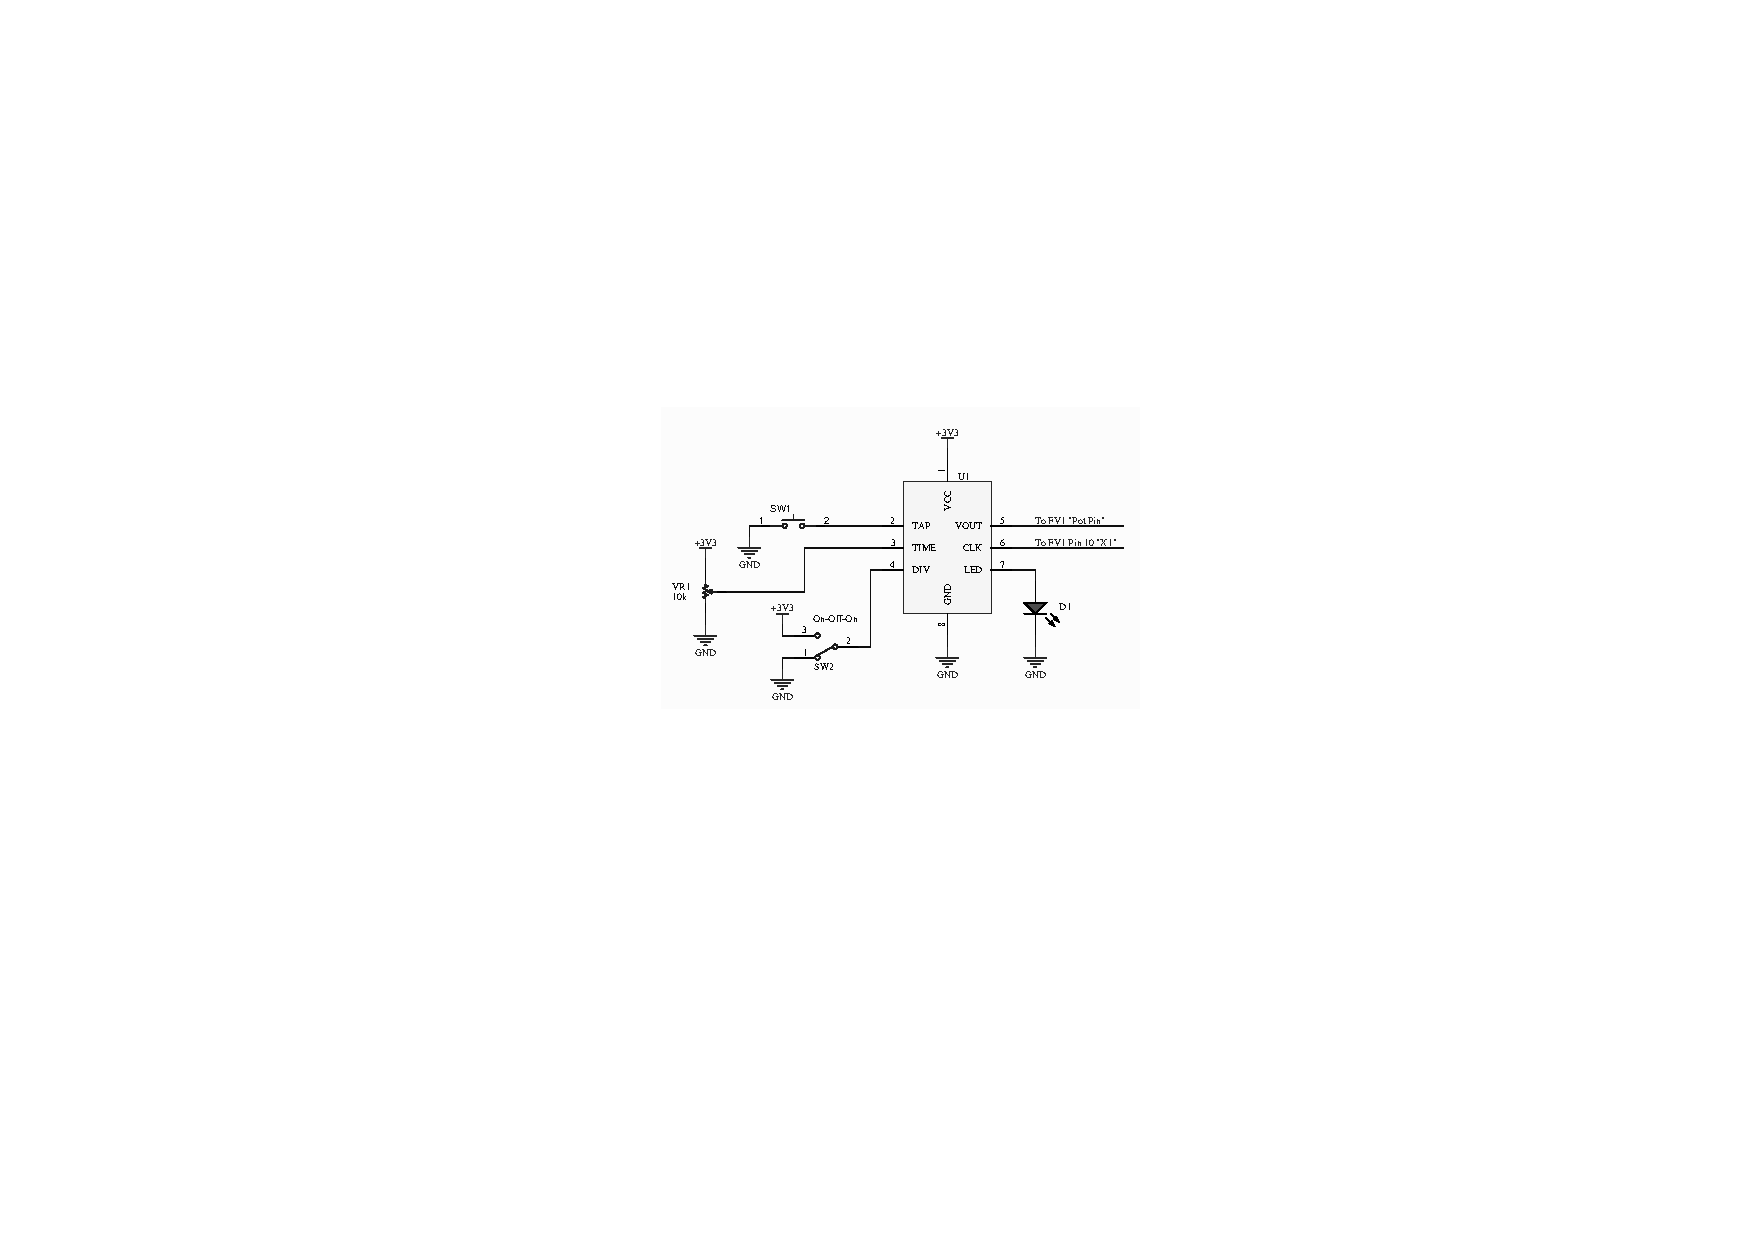
\includegraphics[scale=2]{Schematic}
\label{Schem}
\caption{Typical Application Schematic}
\end{center}
\end{figure}
\vfill
\newpage
\section{Absolute Maximum Ratings}
\bigbreak
\begin{table}[h!]
\centering
\begin{tabular}{|c|c|}
\hline
Storage Temperature	& -65°C to +150°C\\
\hline
Operating Temperature & -40°C to +105°C\\
\hline
Voltage on any pin except pin 6	& -0.5V to Vcc + 0.5V\\
\hline
Voltage on Pin 6 & -0.5V to +13.0V\\
\hline
Power Supply Voltage & -0.5V to +6.0V\\
\hline
I/O Pin sink/source current & -40 to 40mA\\
\hline
DC Current for a supply pin & 100.0mA\\
\hline
\end{tabular}
\caption{Absolute Maximum Ratings}
\end{table}
\bigbreak
\bigbreak
\section{DC Characteristics}
\bigbreak
\begin{table}[h!]
\centering
\begin{tabular}{|c|c|c|c|}
\hline
\rowcolor{lightgray}{\Large\textbf{Parameter}} & {\Large\textbf{Min}} & {\Large\textbf{Max}} & {\Large\textbf{Unit}}\\
\hline
Power Supply Voltage & 1.8 & 5.5 & V\\
\hline
Power Supply Current & 5.8 & 7 & mA\\
\hline
\end{tabular}
\caption{DC Characteristics}
\end{table}
\bigbreak
For any other DC characteristics please refer to the ATtiny402 \href{http://ww1.microchip.com/downloads/en/DeviceDoc/ATtiny202-402-AVR-MCU-with-Core-Independent-Peripherals_and-picoPower-40001969A.pdf}{\underline{datasheet}} (p.476).
\bigbreak
\bigbreak
\section{Specifications}

\begin{table}[h!]
\centering
\begin{tabular}{|c|c|c|c|}
\hline
\rowcolor{lightgray}{\Large\textbf{Parameter}} & {\Large\textbf{Min}} & {\Large\textbf{Max}} & {\Large\textbf{Unit}}\\
\hline
Delay Time & 0 & 1000 & ms\\
\hline
PWM frequency & - & 20 & kHz\\
\hline
Clock frequency & - & 48 & kHz\\
\hline
All Potentiometer/Toggle Input & 0 & Vcc & V\\
\hline
\end{tabular}
\caption{Specifications}
\end{table}

All specifications tested at VCC = 3.3V.

\section{Power Supply}
\bigbreak
In order to function properly the module \textbf{must} be powered from the same 3.3V power supply than the FV1. Any voltage difference between the FV1Buddy and the FV1 power supplies will introduce some time error between the tap tempo and the delay.
A 0.1$\mu$F capacitor between Vcc and GND is already included in the module. Additional decoupling shouldn't be necessary.\\

\section{Calibration}
\label{sec:calib}
\bigbreak
The FV1Buddy comes with a 1000ms maximum delay. However some FV1 delay programs have a smaller maximum delay to accommodate the FV1 performance characteristics.\\
The FV1Buddy module maximum delay can be adjusted to 700, 800, 900 or 1000 ms.\\

To to calibrate the FV1Buddy, follow these instructions :\\
\begin{itemize}
\item Make sure the module is powered down.
\item Position the Time potentiometer to the desired maximum delay.
\item Minimum for 700ms, 10 o'clock for 800ms, 2 o'clock for 900ms, maximum for 1000ms.
\item Press the Tap Button.
\item Power Up the FV1Buddy while keeping the Tap Button Pressed.
\item Keep the button pressed while the Tempo LED blinks twice.
\item Release the Tap Button.
\item The LED blinks twice, the module is now calibrated to the new maximum delay.\\
\end{itemize}

\newpage
\section{Controls}
\subsection{Tap Tempo Button}
\bigbreak
This input is only compatible with a momentary switch.
The debounce is handled by software and with a 0.1$\mu$F capacitor in parallel to the Switch. No extra external components have to be used.\\

The program starts counting milliseconds after the first press. The delay time tapped is in effect right after the second press of the tap button. After the second press of the tap button, every following tap in the sequence is averaged in order to reach easily the desired tempo. 

If the button is not pressed again after a certain time ,the timer is reset and the tap sequence is ended. When a tap sequence has started, it will take 2 pulsations to be finished (the LED will start blinking on its own).\\

If the tap tempo button is pressed only once, the tap sequence will be aborted after the reset time passed.\\
The reset time follows this equation: $\frac{Max Delay}{Tempo Div Mult} + 800 = Reset Time (ms)$\\

Max Delay is either 1000, 900, 800 or 700ms. Tempo Div Mult is the multiplier of the current time division (1, 0.75, 0.5, 0.33, 0.25, 0.17).\\

When the tap tempo is active, the tempo LED will blink with the rhythm you tapped, regardless of the selected tempo division.\\

\subsection{Delay Time}
\label{subsec:delaytime}
\bigbreak
This input is to voltage control the delay time. This input will control the delay time until you activate the tap tempo. While the delay time is controlled by this input, the Tempo LED and will stay on.\\

To take back control from the Tap Tempo, you just need to modify this input's voltage by 7\%. Typically, you would use a Potentiometer for the delay time control. The recommended potentiometer value is 10k$\Omega$ or above, to avoid having too much current going through the pin.\\

You can add a 0.1$\mu$F capacitor between the input and ground for smoother time changes.\\

\subsection{Tempo Division Select}
\label{subsec:tempodiv}
\bigbreak
Six different tempo division are accessible with this input. To access every time division a SPDT On-Off-On toggle switch is required.\\

The first three time divisions are fourth, dotted eighth and eighth. The last three time divisions are accessed by first pressing the tap button and then changing the toggle position while the tap button is pressed. The press will not count as a press for the tap tempo. The three last time divisions are triplet, sixteenth and sextuplet.\\

The time divisions are selected by changing the Tempo Div Select Pin's voltage (Pin 4).\\

If the time division is changed while the Tap Tempo is active, the delay time will be changed accordingly instantly.\\

On the module, the middle position is accessed by putting a 27k$\Omega$ resistor between pin 4 and ground.\\

\subsection{Ramp Modulation}
\label{subsec:ramp}
\bigbreak
A ramp modulation can be activated if the tap button is pressed more than 2 seconds.\\
The ramp will begin to ascend then will descend once the max delay is achieved.\\
The modulation speed can be controlled by moving the Time Potentiometer accordingly. The movements won't be taken into account once you release the tap button.\\

\section{Tempo Save}
\label{sec:temposave}
\bigbreak
When you tap a tempo it is saved on the FV1Buddy's EEPROM. This means that if you power down the FV1Buddy while a tap sequence is active, the module will resume this sequence when powered up. This is true even if some parameters are moved when the FV1Buddy is powered down.\\

\section{Vout}
\label{sec:vout}
\bigbreak
The voltage output of pin 5 is to be connected to one of the "pot" inputs of the FV1 DSP (pins 20, 21 \& 22).\\
This analog voltage is achieved by passing a 20kHz PWM through an onboard RC low-pass filter. The low-pass filter is composed of a 10k$\Omega$ resistor and a 10$\mu$F capacitor.\\

\section{Clock Output}
\label{sec:clock}
\bigbreak
The clock output of pin is to be connected to the "X1" pin of the FV1 DSP (pin 10).\\
The clock has a frequency of 48kHz and will expand the bandwidth of the DSP up to 24kHz comparing to a 15kHz bandwidth with an oscillator.\\
This change will be pretty noticeable and help you fully appreciate your audio effects.\\

\section{Tempo LED}
\label{sec:led}
\bigbreak
When the delay time is controlled by the Time Potentiometer the LED will stay on.\\
When tapping a tap sequence, the LED will blink exactly when you press the tap button, beginning with the second press.\\
When the Tap Tempo is active, the tempo LED will blink in sync with the tempo you tapped regardless of the tempo division selected.\\
A 1k$\Omega$ current limiting resistor is included on the module.

\end{document}